\begin{figure}[ht]
	\centering
	\footnotesize

	\psfrag{oh}[c][c] {$O$}

	\psfrag{u}[c][c] {$u$}
	\psfrag{fu}[c][c] {$f(u)$}

	\psfrag{fuR}[c][c] {$f(u_{R})$}
	\psfrag{fuL}[c][c] {$f(u_{L})$}

	\psfrag{uR}[c][c] {$u_{R}$}
	\psfrag{uL}[c][c] {$u_{L}$}

	\psfrag{fpuR}[c][c] {$f'(u_{R})$}
	\psfrag{fpuL}[c][c] {$f'(u_{L})$}

	\psfrag{cvLR}[c][c] {$\text{Convex: } u_{L} > u_{R}$}
	% \psfrag{cvRL}[c][c] {$\text{Convex: } u_{L} > u_{R}$}

	\psfrag{ccLR}[c][c] {$\text{Concave: } u_{L} < u_{R}$}
	\psfrag{ccRL}[c][c] {$\text{Concave: } u_{L} > u_{R}$}

	\psfrag{sfu}[c][c] {$[f]/[u]<0$}

	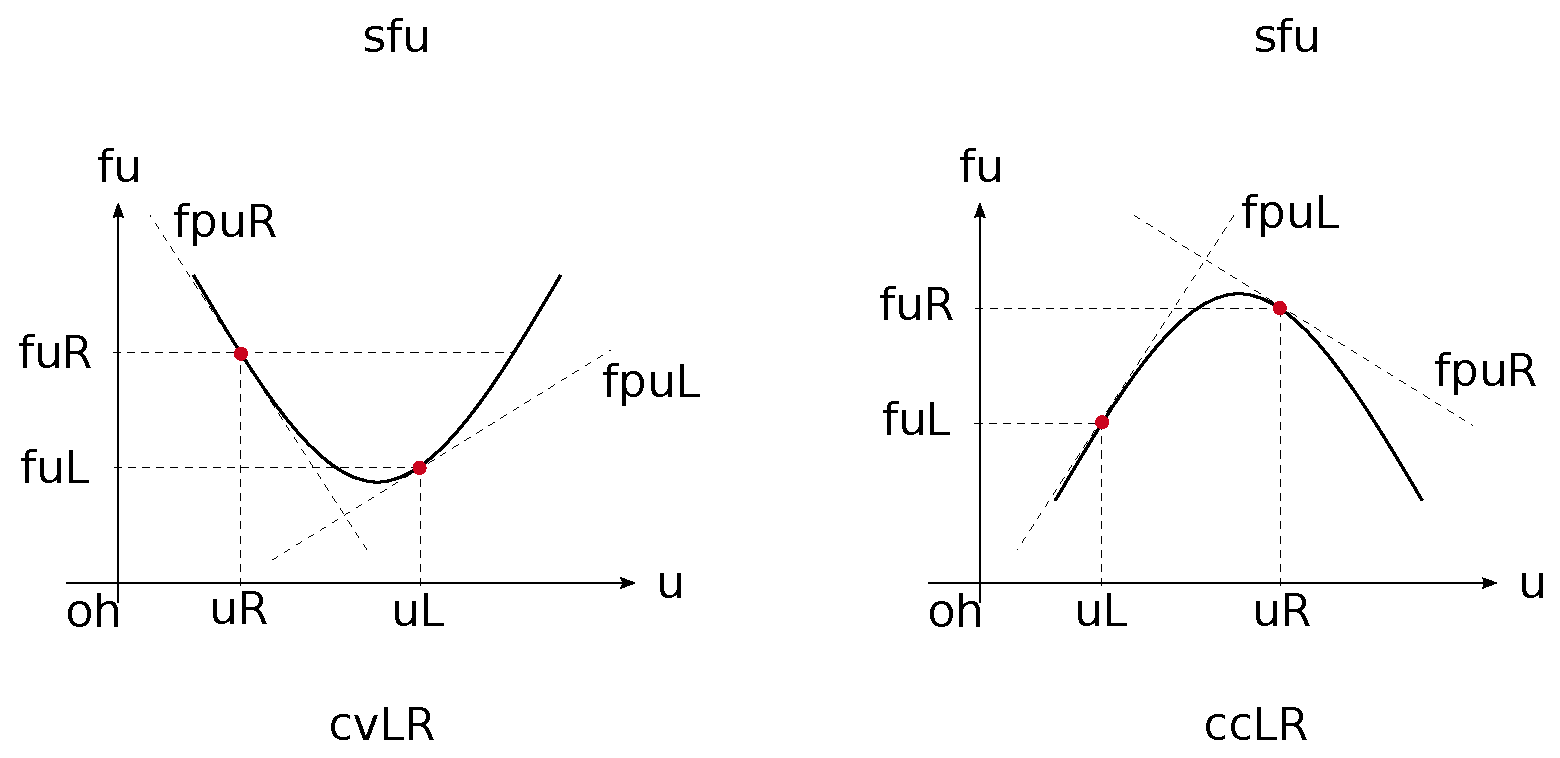
\includegraphics[width=0.99\textwidth]{convexityfu_case22.eps}
	\caption{Case 2.2:
	Convexity and concavity for $u_{L} < u_{R}$ and $u_{L} > u_{R}$,
	where the condition $f^\prime(u_L) \geq 0 \geq f^\prime(u_R) \wedge [f]/[u]<0$
	holds.}
	\label{\LABEL}
\end{figure}